%% Einleitung.tex
%% $Id: einleitung.tex 28 2007-01-18 16:31:32Z bless $
%%

\chapter{Einführung}
\label{ch:Introduction}

Weltweit leiden 15\% der Menschen unter Atemaussetzern während des Schlafs, von denen 85\% undiagnostiziert sind.
Heutige Methoden, die es zur Klassifikation solcher respiratorischer Ereignisse gibt, sind aufwendig und kostspielig. 
Zudem gibt es keine Möglichkeit, diese bequem von Zuhause aus durchzuführen.

Es gibt diverse Arten von Atemaussetzern, zum Beispiel die zentrale Apnoe, die Hauptbestandteil dieser Bachelorarbeit ist. 
Bei zentralem Apnoe setzt die Atmung bei geöffneten Atemwegen für mindestens 10 Sekunden aus. 
Der Grund für den Atemaussetzer ist, dass das Gehirn in dieser Zeit dem Körper keine Signale zum Atmen weitergibt.

\begin{figure}[h]
  \centering
  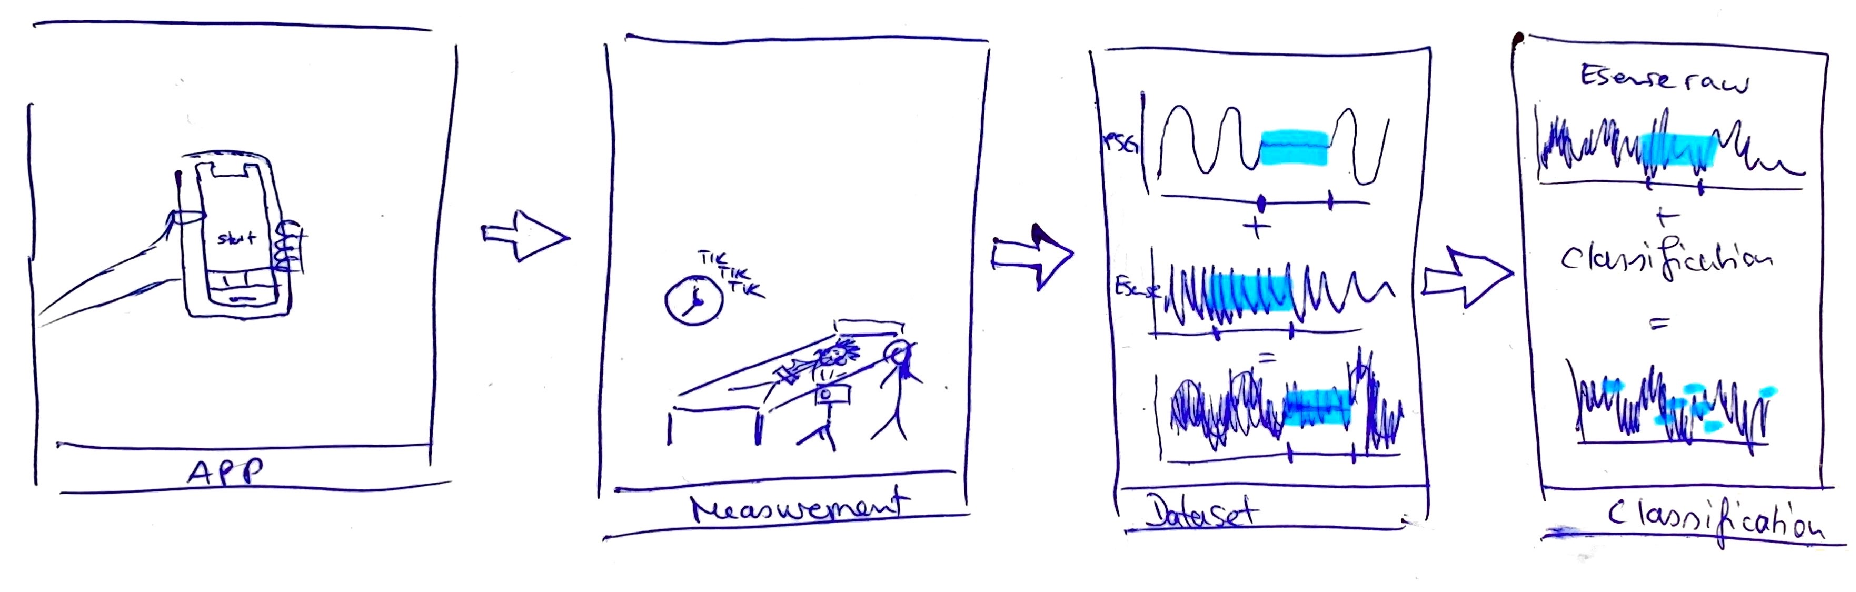
\includegraphics[width=0.3\textwidth]{ba_record}
  \caption{Ablauf der Bachelorarbeit}
  \label{introduction:ba_record}
\end{figure}

Diese Bachelorarbeit fokussiert sich darauf, mittels Earables ein solches zentrales Apnoe zu klassifizieren.
Die eSense Earpods dienen hier als Grundlage.
Sie beinhalten eine inertiale Messeinheit (IMU), womit die nötigen Signale aufgezeichnet werden. 
Der entscheidende Vorteil gegenüber vorherigen Ansätzen ist die Position des Sensors.
Da dieser am Ohr platziert ist, wird ein genaueres Signal als beispielsweise ein am Oberkörper platzierter Sensor.
Somit ist eine Möglichkeit geboten, ein Apnoeereignis im eigenen Bett zuhause zu klassifizieren. 
Zu Beginn der Arbeit wurde eine App erstellt, welche Messergebnisse mit den eSense Earpods während einer Nutzerstudie aufzeichnet.
Während der Nutzerstudie werden die Studienteilnehmer gebeten, an bestimmten Zeitpunkten die Luft für 10, 20 und 30 Sekunden anzuhalten.
Dies simuliert ein zentrales Apnoeereignis und stellt die Grundlage dar, unter welchen der Klassifikator seine Entscheidung trifft.

Die Evaluation wurde mit dem Kreuzvalidierungsverfahren durchgeführt und ergab eine hohe Varianz in den Ergebnissen von Studienteilnehmer zu Studienteilnehmer.
Während ein paar Resultate zu Overfitting neigten, erzielten die restlichen Resultate sehr gute Werte.
